\documentclass{article}

\usepackage{physics}
\setlength{\oddsidemargin}{0 in}
\setlength{\topmargin}{-0.6 in}
\setlength{\textwidth}{6.5 in}
\setlength{\textheight}{8.5 in}
\setlength{\headsep}{0.75 in}
\setlength{\parindent}{0 in}
\setlength{\parskip}{0.1 in}

\usepackage{amsmath,amsfonts,graphicx}
\usepackage[utf8]{inputenc}
\usepackage[english]{babel}
 \usepackage{csquotes}

 \usepackage{graphicx}
\usepackage{subcaption}
\usepackage[
backend=biber,
style=numeric,
sorting=ynt
]{biblatex}
 
\addbibresource{refs.bib}

\begin{document}
\begin{titlepage} % Suppresses displaying the page number on the title page and the subsequent page counts as page 1
		\newcommand{\HRule}{\rule{\linewidth}{0.5mm}} % Defines a new command for horizontal lines, change thickness here
		
		\center % Centre everything on the page
		
		%------------------------------------------------
		%	Headings
		%------------------------------------------------
		
		\textsc{\LARGE Faculty of Engineering - Alexandria University}\\[1.5cm] % Main heading such as the name of your university/college
		
		\textsc{\Large Pattern Recognition}\\[0.5cm] % Major heading such as course name
		

		\HRule\\[0.4cm]
		
		{\huge\bfseries NLP and Sentiment Analysis}\\[0.4cm] % Title of your document
		
		\HRule\\[1.5cm]
		
		%------------------------------------------------
		%	Author(s)
		%------------------------------------------------
		
		\begin{minipage}{0.5\textwidth}
			\begin{flushleft}
				\large
				Abdelrahman Mohamed Abdelnabi
				\texttt{3466} \\
				Ahmed Essam Shaheen
				\texttt{3321} \\
				Amr Mohamed El Sayed
				\texttt{3400} \\
			\end{flushleft}
		\end{minipage}
		~
		\begin{minipage}{0.3\textwidth}
			\begin{flushright}
				\large
				\textit{Supervisor}\\
				Dr. Marwan \textsc{Torki} % Supervisor's name
			\end{flushright}
		\end{minipage}


		\vfill\vfill\vfill % Position the date 3/4 down the remaining page
		
		{\large\today} % Date, change the \today to a set date if you want to be precise
		
		\vfill % Push the date up 1/4 of the remaining page
		
	\end{titlepage}
	
	
	
	\section{Introduction}
	
	We are required to perform sentiment analysis on the IMDB movie reviews dataset. Sentiment analysis classification, as any other classification problem, requires the input datapoints, the reviews in our case to be represented as vectors of real numbers. 
	
	We first apply text pre-processing the to the dataset by tokenizing the reviews, removing stopwords, removing HTML tags, tagging the words with \textit{part of speech} (POS) tags, and finally lemmatizing the tokens.
	
	A challenging task is to convert the a review to a single fixed size vector. We perform vectorization of the documents by trying several models for representing documents as vectors, including traditional and modern models. We try the famous \textit{tf-idf} (term frequency - inverse document frequency) which converts a single review directly into a feature vector. We also try three different forms of modern word embedding technique. The first is using \textit{Genism} to train a word embedding model on our dataset and generate the embeddings for each word in our vocabulary, the second is using pre-trained embeddings such as \textit{word2vec} and \textit{GloVe}, and the third is using \textit{Doc2VecC}, a model that combines embeddings for words in a document by averaging the embeddings of each word in the document in a way similar to tf-idf.
	
	Now we have a feature vector for each document, we can train any classifier and perform sentiment analysis as required.
	
	\section{Text Pre-processing}
	
	The goal of text pre-processing it to clean the text by removing punctuation, stopwords, tokenizing the text and reducing inflectional and derivationally related forms of a word to a common base form (lemmatization).
	
	Pre-processing is expected to increase the accuracy of classification as it removes words that wont have an effect from the input words, for example the word 'the' might be repeated so man times and it wont help in classifying a class from the other, so the role of our pre-processing is to remove these words that add nothing to our model.
	
	We use \texttt{NLTK} to perform text pre-processing.
	
	\section{Text Vectorization}
	
	\subsection{Bag of Words}
	
	Bag of words (BoW) is model for representing text documents as vectors by encoding each document in a one long vector which length is the size of the vocabulary of the corpus. The \textit{i-th} value in the vector represents the frequency of the \textit{i-th} vocabulary word in the document. Such representation is usually sparse since most vector elements are zero and takes up a lot of memory space.
	
	By treating words and phrases as unique and discrete symbols, BoW often fails to capture the similarity between words or phrases and also suffers from sparsity and high dimensionality. \cite{chen2017efficient}
	
	\subsection{TF-IDF}
	
	This is another method which is based on the frequency method but it is different to the count vectorization in the sense that it takes into account not just the occurrence of a word in a single document but in the entire corpus.
	
	Common words like ‘is’, ‘the’, ‘a’ etc. tend to appear quite frequently in comparison to the words which are important to a document. For example, a document A on Machine Learning is going to contain more occurrences of the word “classification" in comparison to other documents. But common words like “the” etc. are also going to be present in higher frequency in almost every document.
	
	Ideally, if a word has appeared in all the document, then probably that word is not relevant to a particular document. But if it has appeared in a subset of documents then probably the word is of some relevance to the documents it is present in.
	
	\subsection{Word2Vec and GloVe}
	
	Word2Vec is a model that learns word embeddings from a corpus by using the fact that similar words usually appear in similar contexts. The model uses a skip-gram or a continuous bag of words to exploit this fact. To try the two different approaches of word embeddings, we use word2vec to learn embeddings of words by feeding it the corpus (excluding test data) and using the pre-trained embeddings of GloVe. Since GloVe is trained on a much larger dataset, it has a slightly higher accuracy as it could learn better embeddings of words and capture its meaning.
	
	\subsection{Doc2VecC}
	
	Doc2VecC is an efficient document representation learning framework, Document Vector through Corruption. Doc2VecC represents each document as a simple average of word embeddings. It ensures a representation generated as such captures the semantic meanings of the document during learning. A corruption model is included, which introduces a data-dependent regularization that favors informative or rare words while forcing the embeddings of common and non-discriminative ones to be close to zero. \cite{chen2017efficient}
	
	Like tf-idf, Doc2vecC favors informative or rare words while forcing the embeddings of common and non-discrimantive ones to be close to zero. This also means that stopwords like \textit{I, The, is, ...} don't have to be removed as they will have a close to zero embedding because of their high frequency of occurrence in the corpus.
	
	The authors of the paper provide the code for their paper on github, along with instructions on how to use it. We downloaded the code and used fed it our pre-processed data including the test and train sets and retrieved the output document vector for each review, which we can then use by feeding it to our desired classifiers. We can also obtain more accurate word embeddings, and therefore more accurate document vectors by feeding the unsupervised part of the dataset as well. This will provide more context for the words to the algorithm which will help it to come up with better word vectors.
	
	\subsection{Doc2Vec}
	Doc2vec modifies the word2vec algorithm to unsupervised learning of continuous representations for larger blocks of text, such as sentences, paragraphs or entire documents.
	
	Since the Doc2Vec class extends gensim’s original Word2Vec class, many of the usage patterns are similar. We can easily adjust the dimension of the representation, the size of the sliding window, the number of workers, or almost any other parameter that you can change with the Word2Vec model.
	
	We found that by concatenating 3 models the accuracy among the test cases increased , we think this is because the number of features has increased and each model is trained on a different set of data. We have also introduced the unsupervised reviews to one of the models to increase the vocab of it and labels in \textbf{doc2vev} are all unique for every input so we assign different and unique labels to these unsupervised reviews. This technique can be seen as ensemble of more than one model to increase accuracy 
	\medskip
	
	
	
	\section{Classification and Supervised Learning}
	
	Figure \ref{fig:tf-idf} shows the classification accuracy when using TF-IDF. Classifiers are tuned on one parameter and cross validated using 10 folds, the bar in the figure represents the variance in the accuracies of each fold, the point represents the mean of the accuracies of the 10 folds. Figure \ref{fig:tf-idf-knn} and \ref{fig:tf-idf-lr} are the results of using TF-IDF on the normalized (cleaned) data after pre-processing. Figure \ref{fig:tf-idf-lr-raw} are the results of TF-IDF on the raw data. Unexpectedly, TF-IDF on the raw data produces better results than when used on the cleaned data.
	
	\begin{figure}
        \centering
        \begin{subfigure}[b]{0.5\textwidth}
            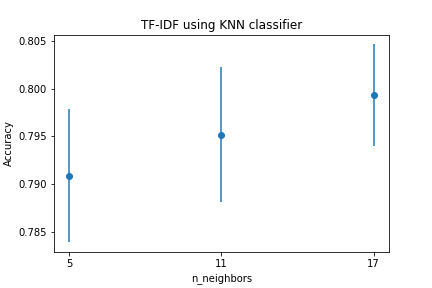
\includegraphics[width=\textwidth]{tf-idf-knn.png}
            \caption{Using a KNN classifier}
            \label{fig:tf-idf-knn}
        \end{subfigure}
        \begin{subfigure}[b]{0.5\textwidth}
            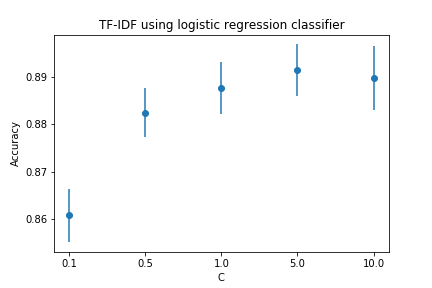
\includegraphics[width=\textwidth]{tf-idf-lr.png}
            \caption{Using a logistic regression classifier}
            \label{fig:tf-idf-lr}
        \end{subfigure}
        
        
        \begin{subfigure}[b]{0.7\textwidth}
            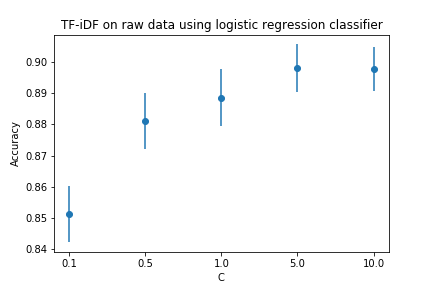
\includegraphics[width=\textwidth]{tf-idf-raw-lr.png}
            \caption{Using a logistic regression classifier on raw data (un-normalized)}
            \label{fig:tf-idf-lr-raw}
        \end{subfigure}
        
        \caption{TF-IDF vectorization of documents and sentiment analysis results using several classifiers}\label{fig:tf-idf}
    \end{figure}
    
    
    \begin{figure}
        \centering
     
        \begin{subfigure}[b]{0.5\textwidth}
            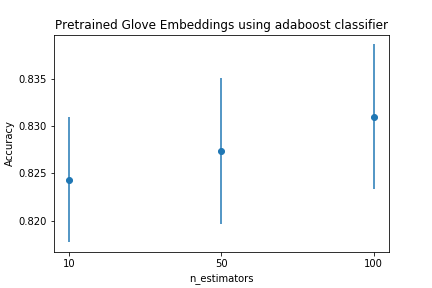
\includegraphics[width=\textwidth]{glove-ada.png}
            \caption{GloVe vectors of documents classified using adaboost}
            \label{fig:glove-ada}
        \end{subfigure}
        
        \begin{subfigure}[b]{0.5\textwidth}
            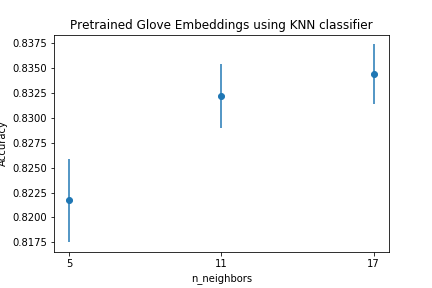
\includegraphics[width=\textwidth]{glove-knn.png}
            \caption{GloVe vectors of documents classified using KNN}
            \label{fig:glove-knn}
        \end{subfigure}
        
        \begin{subfigure}[b]{0.5\textwidth}
            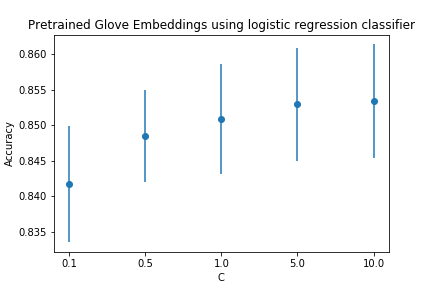
\includegraphics[width=\textwidth]{glove-lr.png}
            \caption{GloVe vectors of documents classified using logistic regression}
            \label{fig:glove-lr}
        \end{subfigure}
        
        \caption{sentiment analysis results using several classifiers using GloVe vectors of documents}\label{fig:glove}
    \end{figure}
    
    
    \begin{figure}
        \centering
        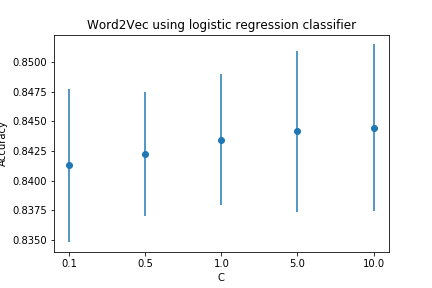
\includegraphics{word2vec-lr.png}
        \caption{Word2Vec tested on logistic regression classifier}
        \label{fig:word2vec}
    \end{figure}
	
	\section{The Big Picture}
	
	\subsection{Effect of Pre-processing}
	
	\subsubsection{Vectorization of Raw Data}
	
	To analyze the effect of preprocessing, we try tf-idf vectorization of documents on the raw data. As figure \ref{fig:tf-idf-lr-raw} shows, the accuracy of tf-idf on the raw the data is marginally higher than that on the normalized data. tf-idf will already handle stop-words and punctuation by giving them a low weight since they appear a lot in the text, however, the fact that the accuracy still increases even without using lemmatization is still confusing to us.
	
	\subsubsection{Selection of Biased Words}
	
	A large amount of the vocabulary appears with about the same percentage in both the positive and negative reviews. Such words are unbiased and have no say in the sentiment of the review in general. Some example of these words from the corpus are \textit{character, saturday, fill, sub-plot, little, typically, instruction, borrow, teenager}. We can focus more on the biased words that are more likely to have a specific sentiment by removing the unbiased words that appear about the same percentage and hence the same frequency since the classes are of the same size in the dataset.
	
	We define a \textit{margin} that decides if a word is biased or unbiased if it appears in both classes. words that appear with a frequency $f$ in the positive class of reviews has to appear with a frequency less than $margin\times f$ in the negative class for this word to be selected as a biased (positive in this case) word. And the same applies for a negative biased word. Increasing the margin will make the process more selective in choosing biased words.
	
	However, words that appear with the same percentage could also include some critical words that usually appears in the context of movie reviews regardless of whether the movie was good or bad. Such words include \textit{likely, worthy, tension, sacrifice, shock, suspense}. It is usually the context that decides how the sentiment. for example \textit{The movie had a lot of tension and suspense} is positive but \textit{The movie did not have any kind of suspense} is negative. We ignore such cases as they are very hard to analyze and are very few in occurrence.
	
	
	\subsection{Feature Choice}
	
	Word embeddings have a specific length that can be tuned, usually longer vectors are better but that is not usually the case. We tried GloVe embeddings on 50 and 300 dimensions. The accuracy in the first case was about 75\% and reached about 84\% in the latter case. Since we are using pre-trained GloVe embeddings, we are constrained to the vector lengths of the GloVe dataset. Similar results should be observed when using Word2Vec (either trained on the dataset or pre-trained).
	
	
	\subsection{Classifier Choice}
	SVM in most cases is the best classifier but it takes huge time to train, logistic regression sometimes work good for high dimensions as data become linearly separable other classifiers like KNN is not practical at all to use. Also, the logistic regression classifier was found to give very high results across the different methods of vectorization.
 
\printbibliography
	
	
\end{document}}
